\newcommand{\changedinc}{\kw{Changed}}
\newcommand{\cut}{\kw{CUT}}
\newcommand{\imr}{\kw{IMR}}
\newcommand{\imrs}{\kw{IMRs}}
\newcommand{\fb}{\kw{FBM}}
\newcommand{\bs}{\kw{BS}}
\newcommand{\fs}{\kw{FS}}
\newcommand{\bfc}{\kw{BF}}
\newcommand{\upl}{\kw{UP}}
%\newcommand{\fbm}{\kw{FBM}}
\newcommand{\fbmatstruct}{\kw{FBMatStruct}}
\newcommand{\matchindex}{\kw{MatStaIndex}}
\newcommand{\matchimr}{\kw{MatchIMR}}
\newcommand{\for}{\kw{FOR}}
\newcommand{\while}{\kw{WHIlE}}
\newcommand{\allmatch}{\kw{mat}}
\newcommand{\affnode}{\kw{affnode}}

\newcommand{\ms}{\kw{SHOUDfs}}
\newcommand{\ballfilter}{\kw{SHOUDbfc}}

\newcommand{\dens}{\kw{den}}
\newcommand{\identifyaffball}{\kw{IdABall}}
\newcommand{\patedgeinsert}{\kw{patEIns}}
\newcommand{\incmatch}{\kw{IncMatch}}
\newcommand{\wmatchindex}{\kw{wMatStaCode}}
\newcommand{\cflag}{\kw{cflag}}
\newcommand{\dflag}{\kw{dflag}}
\newcommand{\gflag}{\kw{gflag}}
\newcommand{\rflag}{\kw{rflag}}

\newcommand{\incgrpat}{\kw{kPatIncGPM}}
\newcommand{\incgrdata}{\kw{kDataIncGPM}}
\newcommand{\dyngr}{\kw{kDynGPM}}
\newcommand{\affballx}{\kw{AffB}}
\newcommand{\affballsx}{\kw{AffBs}}
\newcommand{\affballacc}{\kw{AffBall^{acc}}}
\newcommand{\affballaccs}{\kw{AffBalls^{acc}}}
\newcommand{\affballimr}{\kw{AffBall^{imr}}}
\newcommand{\affballimrs}{\kw{AffBalls^{imr}}}
\newcommand{\patinc}{\kw{dynamicPG}}
%\newcommand{\patinc}{{\sc dynPG}\xspace}
%\newcommand{\datainc}{{\sc dynDG}\xspace}
\newcommand{\datainc}{\kw{dynamicDG}}
\newcommand{\optpatinc}{\kw{SHOULDoptinc}}
\newcommand{\inc}{\kw{dynamic}}
\newcommand{\matchs}{\kw{R}}
\newcommand{\comb}{\kw{combine}}
\newcommand{\optinc}{\kw{optDynamic}}

\newcommand{\incp}{\kw{dynamicP}}
\newcommand{\incd}{\kw{dynamicG}}


\section{A Unified Incremental Solution}
\label{sec-dynamictopk}

In this section, we first analyze the challenges and design principles of dynamic top-$k$ team formation,
and then develop a unified incremental framework for \dynteamF.
For convenience, the notations used are summarized in Table~\ref{tab-notation}.


\subsection{Analyses of Dynamic Team Formation}


By Theorem~\ref{thm-tsim-radius}, pattern $P$ matches a ball $\ball{[v, t]}$ ($t \in [1,r-1]$), only if $P$ matches ball $\ball{[v, r]}$ via graph simulation,
and the match results for $\ball{[v, t]}$ can be derived from the matches for $\ball{[v, r]}$.
Therefore, the key of the incremental computation is to deal with the balls $\ball{[v, r]}$ with radius $r$.
In the sequel, a ball has a radius $r$ by default.

%Moreover, incremental algorithms typically maintain some auxiliary data structures, which are specifically designed for the update types and need to be maintained by the incremental algorithms. An incremental algorithm for \dyngr should be able to design auxiliary structures to store information needed for both pattern and data increments and maintain it for future ({\em both}) pattern and data increments. This raises even more challenges in designing incremental algorithms for \dyngr, compared to those for \incgrpat and \incgrdata alone.

\eat{%%%EAT
Like data incremental problems, it would be nice to have {\em bounded incremental algorithms}~\cite{Reps96} for pattern incremental problems, which are a class of incremental algorithms whose time complexity depends on the sizes of $P$ and $\changedinc$, which is the changes to the input and output only (\ie $\Delta P$ and the difference between $PG_k(P, G)$ and $PG_k(P\oplus\Delta P, G)$),
and is independent of the size of $G$ and $PG_k(P, G)$.
However, due to the inherent difference between pattern increments and data increments, and the presence of top-$k$ semantic, they are not available for \incgrpat, as shown below.
We say an incremental problem is bounded if it has a bounded incremental algorithm described as above, and is unbounded otherwise.

Similar to the negative results in \cite{FanLMTWW10,FanWW13-tods}

The following results show that even we consider pattern or data increments alone, traditional bounded incremental algorithms are not available for \dyngr already.

%\begin{theorem}
%\label{thm-inc-grouprec-pat}
%$\incgrpat(P,G,k,PG_k(P,G),\Delta P)$ is unbounded, even when
%\bi
%\item $\Delta P$ is
%(a) a single-edge insert,
%(b) a single-edge delete,
%(c) a single-node insert,
%(d) a single-node delete, or
%(e) a single-node-capacity change;
%\item $k$ is 1 or $n$, where $n$ is the number of nodes in $G$.
%\ei
%\end{theorem}
%
%Moreover, due to the presence of top-$k$ semantic, the bounded incremental property is not available for \incgrdata either, as shown below.
%
%\begin{theorem}
%\label{thm-inc-grouprec-data}
%$\incgrdata(P,G,k,PG_k(P,G),\Delta G)$ is unbounded, even when
%\bi
%\item $\Delta G$ is
%(a) a single-edge insert,
%(b) a single-edge delete,
%(c) a single-node insert,
%(d) a single-node delete, or
%\item $k$ is 1 or $n$, where $n$ is the number of nodes in $G$.
%\ei
%\end{theorem}

}%%%EAT

We first analyze the inherent computational complexity of the dynamic top-$k$ team formation.

\stitle{Incremental complexity analysis}. As observed in~\cite{Reps96,inc-survey}, the complexity of incremental algorithms should be measured by the size $|\aff|$ of {\em the changes} in the input and output, rather than the entire input, to measure the amount of work essentially to be performed for the problem.

An incremental problem is said to be {\em bounded} if it can be solved by an algorithm whose complexity is a function of $|\aff|$ alone, and is {\em unbounded}, otherwise. Unsurprisingly, the dynamic top-$k$ team formation problem is unbounded, similar to the other extensions of graph simulation \cite{FanLMTWW10,FanWW13-tods}.


\begin{prop}
\label{thm-inc-grouprec-pat}
The \dynteamF{} problem is unbounded, even for $k$ = 1 and unit pattern or data updates.
\end{prop}


We then illustrate the impact of pattern and data updates on the matching results with an example.


\begin{example}
\label{exm-pattern-challenge}
Continue Example~\ref{exm-motivation-inc} with $\Delta P_1$ and $\Delta G_1$.

% that obviously may introduce new matches.
%For convenience of presentation, we treat $\Delta P_1$ and $\Delta G_1$ separately.

\sstab
(1) For $\Delta P_1$, $\ball{[\kw{PM_1}, 2]}$ already matches $P$, and may produce more matched nodes for $P_1\oplus \Delta P_1$,
thus a re-computation for perfect subgraphs is needed.
For all other balls, $\Delta P_1$ may turn unmatched nodes to matched and may produce perfect subgraphs,
thus re-computation is also needed.

\sstab
(2) For $\Delta G_1$, it produces a new perfect subgraph for $P$ in $G_1\oplus\Delta G_1$,
\ie the connected component having \kw{PM_2}.
%The question is how to directly find new and maintain previous answers without redundant computation.
\end{example}

%\subsection{Analyses of Challenges}
%\label{subsec-challenges}


\begin{table}[tb!]
	%\vspace{-2ex}
	%\vspace{2ex}
	\begin{center}
		\begin{small}
			%\vspace{-2ex}
			\scriptsize
			\begin{tabular}{|c|l|}
				\hline
				{\bf Notations}             &  {\bf Description}     \\
				\hline\hline
				$P,G$                     &  pattern and data graphs       \\ \hline
				$\ball{[v, r]}$              &  a ball in $G$ with center node $v$ and radius $r$  \\ \hline
				$L_k(P, G)$                  &  the list of top-$k$ perfect subgraphs in $G$ for $P$  \\ \hline
				$\Delta P, \Delta G$       &  pattern and data updates       \\ \hline
				$\oplus$                    &  applying updates $\Delta P$ and $\Delta G$ to $P$ and $G$       \\ \hline
				${\cal P}_{h}=\{P_{fi}, C\}$     &  pattern fragmentation: $h$ fragments and cut    \\ \hline
				$\affballsx$                &  affected balls       \\ \hline
				$M(P_{fi}, \ball{[v,r]})$    &  the maximum match relation in $\ball{[v,r]}$ for $P_{fi}$   \\ \hline
				$\tilde{M}(P,G)$            &  fragment-ball matches (auxiliary structure)     \\ \hline
				$\fs$, $\bs$              &  fragment status, ball status (auxiliary structure) \\    \hline
				$\fb$                       &  fragment-ball-match index, containing $\fs, \bs$ \\    \hline
				$\bfc$, $\upl$              &  ball filter, update planner (auxiliary structure) \\    \hline
			\end{tabular}
			\vspace{-1ex}
		\end{small}
		\caption{Notations}
		\label{tab-notation}
		\vspace{-6ex}
	\end{center}
\end{table}


We finally discuss the challenges and principles of designing incremental algorithms for \dynteamF{} from three aspects.

%impacts of pattern and data updates, maintenance of proper auxiliary information, and support of simultaneous pattern and data updates.


\stitle{(1) Impacts of pattern and data updates}.
Beyond Proposition~\ref{thm-inc-grouprec-pat} and Example~\ref{exm-pattern-challenge}, one can also verify that (a) unit pattern updates are likely to result in the entire change in previous results, such that all balls need to be accessed and all matches need to be re-computed,
and (b) the impact of data updates can also be global, such that the entire data graph may need to be accessed to re-compute matches.
Hence, the key is to identify and localize the impacts of pattern and data updates.

%It is rather better to identify the changes in match results in response to data updates, to minimize unnecessary recomputation.
%However, the identification can be difficult and time-consuming.
%It is crucial to identify which parts of $G$ are affected by the data updates and updates match results only within them.
%However, the identification can be difficult and time-consuming.
%The number of affected balls may vary with different data updates.


\stitle{(2) Maintenance of auxiliary information}.
Auxiliary data on intermediate or final results for $P$ in $G$ are typically maintained for incremental computation \cite{Reps96,FanWW13-tods}.
How to design light-weight and effective auxiliary structures is critical.
One may want to store $M(P,G)$, the match relations of $P$ for all balls in $G$,
as adopted by existing incremental pattern matching algorithms for data updates \cite{FanWW13-tods}.
However, the impact of $\Delta P$ is global, as shown in Example~\ref{exm-pattern-challenge}.
By storing $M(P,G)$, for pattern edge/node deletions, it has to recompute matches for all balls, \ie the entire $M(P,G)$.
Thus, storing $M(P,G)$ could be useless, not to mention $L_{k}(P,G)$, the list of top-$k$ perfect subgraphs for $P$ in $G$ \wrt $M(P,G)$.

\stitle{(3) Support of continuous pattern and data updates}.
%Previous research on incremental problems typically focus on increments to the data parts instead of the queries,
%and if exist, the dynamic algorithms either support pattern or data updates, not both of them~\cite{MottinGReform15,FanWW13-tods}.
A practical solution should support continuous pattern and data updates, separately and simultaneously, which further increases difficulties on the design of auxiliary data structures and incremental algorithms.

\subsection{Unified Incremental Framework}
%\label{subsec-framework}

Nevertheless, we develop an incremental approach to handling pattern and data updates in a unified framework, by utilizing {\em pattern fragmentation} and {\em affected balls} to localize the impacts of pattern and data updates, and to reduce the cost of maintaining auxiliary structures and computations.

%In light of the challenges, it is desirable to devise a unified efficient incremental approach to handle both $\Delta P$ and $\Delta G$,
%which can reduce the cost for maintaining auxiliary structures and computing final results,
%by restricting the update impacts from global to local.
%Therefore, we propose the {\em dynamic top-$k$ graph pattern matching} model to solve \dynteamF\.
%\looseness=-1

\stitle{(1) Localization with pattern fragmentation}. 
We say that \{$P_{f1}(V_{f1},V_{f1})$, $\ldots$, $P_{fh}(V_{fh},V_{fh})$, $C$\} is an {\em $h$-fragmentation} of pattern $P(V_{P}$, $E_{P})$, denoted as ${\cal P}_{h}$,
if (1) $\bigcup_{i=1}^{h}V_{fi}=V_{P}$, (2) $V_{fi}\cap V_{fj} = \emptyset$ for any $i\ne j\in[1, h]$,
(3) $E_{fi}$ is exactly the edges in $P$ on $V_{fi}$, and (4) $C=E_P \setminus (E_{f1}\cup\ldots\cup E_{fh})$.

We also say $P_{fi}$ ($i\in[1,h]$) as a {\em fragment} of $P$, and $C$ as a {\em cut} of $P$, respectively.

Observe that by pattern fragmentation, a pattern update on $P$ is either on a fragment $P_{fi}$ or on the cut $C$ of $P$, and, in this way, the impact of pattern updates is localized. Moreover, graph simulation holds a nice property on pattern fragmentation, as shown below.

\vspace{-0.5ex}
\begin{theorem}
\label{thm-compose}
Let $\{P_{f1},\ldots,P_{fh}\}$ be an $h$-fragmentation of pattern $P$.
For any ball $\ball{}_i$ in $G$, let $M_i$ ($i\in[1,h]$) be the maximum match relation in $\ball{}_i$ for $P_{fi}$ via graph simulation,
and $M$ be the maximum match relation in $\ball{}_i$ for $P$ via graph simulation, respectively,
then $M\subseteq\bigcup_{i=1}^{h}M_{i}$.
\end{theorem}

We also say that $M_i$ is a {\em partial match relation} in ball $\ball{}_i$ for $P$ via graph simulation.
%By Theorem~\ref{thm-compose}, instead of computing $M$ in $\ball{}$ \wrt\ $P$ directly, we can compute $M$ by first computing each $M_i$ in $\ball{}$ \wrt\ $P_{fi}$,
%and then combining them together.
By the nature of graph simulation~\cite{infsimu95}, $\bigcup_{i=1}^{h}M_{i}$ is actually an intermediate result of $M$.
%such that the method above does not incur additional computation cost.
Once we have the maximum match relation $M$ for $P$ in $\ball{}_i$, via graph simulation, we can further produce the result for $P$ in  $\ball{}$ via team simulation, by a capacity check.

That is, based on pattern fragmentation, we maintain 
an auxiliary structure for storing fragment-ball matches for incremental computations,
\ie $\tilde{M}(P,G)$ \wrt ${\cal P}_{h}$ that is the maximum match relations for all pattern fragments of $P$ in all balls of $G$, via graph simulation.
Moreover, its space cost is light-weight, as will be shown in the experimental study.
%\revise{
%Moreover, by Theorem~\ref{thm-tsim-radius}, the match results in balls $\ball{[v, t]}$ ($1 \leq t < r$) can be easily derived from the %matches in ball $\ball{[v, r]}$.
%Thus, we only store the maximum match relations for all pattern fragments of $P$ in the balls with radius $r$ of $G$.}
%which will be shown to be much more informative than storing $M(P,G)$ and $L_{k}(P,G)$.
%Its space cost is light-weight, and takes 25MB only, together with all indexes for \citationd that needs 36MB to store itself.


%Indeed, it only takes 25MB and 65MB to store $\tilde{M}(P,G)$ along with all other indexes for Citation and YouTube,  which need 36MB and 114MB, respectively, for storing the entire data graphs.

%We already know that pattern updates $\Delta P$ on $P$ can be treated as the updates $\Delta P$ on $P_{fi}$ or $C$ of $P$.
%If we have cached the maximum match relations of all pattern fragments,
By storing $\tilde{M}(P,G)$, we have $\bigcup_{i=1}^{h}M_{i}$ for each ball $\ball{}$,
and we can simply update $M_i$ while leaving other parts untouched. That is, we indeed compute for $P_{fi}\oplus\Delta P(\ball{})$, instead of $P\oplus\Delta P(\ball{})$, and combine all $P_{fi}\oplus\Delta P(\ball{})$ derive $P\oplus\Delta P(\ball{})$.
Even better, the updates $\Delta P$ on $C$ of $P$ only involve with a simple combination process, avoiding the computation for any pattern fragments.


For a better incremental process, we typically want (1) to avoid skewed updates by balancing the sizes of all fragments, and (2) to minimize the efforts to assemble the partial matches of all fragments.
Thus we define and investigate the {\em pattern fragmentation} problem. 

Given pattern $P$ and a positive integer $h$, it is to find
an $h$-fragmentation of $P$ such that both $\max(|P_{fi}|)$ ($i\in[1,h]$) and $|C|$ are minimized.
Intuitively, the bi-criteria optimization problem partitions a pattern into $h$ components of roughly equal size while minimizing the cut size.

\eat{%%%EAT2017-8-2}
Given $P$ and a positive integer $h$, the {\em pattern fragmentation}  problem is to find
an $h$-fragmentation of $P$ such that both $\max(|P_{fi}|)$ ($i\in[1,h]$) and $|C|$ are minimized.
%
Intuitively, we want (1)  to avoid skewed updates by making all fragments roughly the same size and (2) to  minimize the efforts to assemble the partial matches of all fragments.
}%%%EAT2017-8-2

The problem is intractable, as shown below.

\vspace{-0.5ex}
\begin{prop}
	\label{prop-fragmentation}
	The pattern fragmentation problem is \NP-complete, even for $h$ = 2.
\end{prop}



However, $P$ and $h$ are typically small in practice~\cite{FanLMTWW10}, \eg $|P|=15$ and $h=3$.
In light of this, we give a heuristic algorithm, denoted by \kw{PFrag}, for the problem, and is shown in the
full version~\cite{fullvldb18}.
\kw{PFrag} works by connecting pattern fragmentation to the widely studied {\sc $(k, \nu)$-Balanced Partition} problem \cite{AndreevR06},
which is not approximable in general, but has efficient and sophisticated heuristic algorithms~\cite{metis-KarypisK98a}.




\stitle{(2) Localization with affected balls (\affballsx)}.
We further localize the impact of pattern and data updates  with {\em affected balls} to avoid unnecessary computations.


We say that a ball in $G$ is {\em affected} \wrt an incremental algorithm \algorithm{A}, and pattern and data updates,
if \algorithm{A} accesses the ball again.
We use $||\affballsx||$ and $|\affballsx|$ to denote the cardinality and total size of \affballsx, respectively.

%We say that a ball is {\em affected} \wrt an incremental algorithm \algorithm{A} and a set of pattern and data updates if \algorithm{A} re-constructs the ball again using the data graph.

%
Indeed, \affballsx are those balls with a possibility to have final results \wrt $\Delta P$ and $\Delta G$.
We only access \affballsx, and ignore the rest balls.
Specifically, (1) for $\Delta P$, it allows us to avoid computing updated partial relations for an updated fragment in every ball;
and (2) for $\Delta G$, the locality property of team simulation supports to localize the update impacts to a set of balls whose structures are changed by $\Delta G$.
%we just do the computation for the balls whose structure is changed due to $\Delta G$.
\looseness=-1

%\stitle{Remark}. By pattern fragmentation and affected balls, we essentially localize the impact of pattern and data updates from the entire to a fraction of $P$ and from all to a subset of balls in $G$ for team simulation.


%\vspace{-0.5ex}
\stitle{(3) Algorithm framework}. We now provide a unified incremental algorithm to handle both pattern and data updates,
based on pattern fragmentation and affected balls.


Given pattern $P$ with its $h$-fragmentation ${\cal P}_{h}$, data graph $G$, two integers $r$ and $k$,
and auxiliary structures (to be introduced in Section \ref{sec-IncAlg}) such as the partial match relations for all pattern fragments and all balls (radius $r$),
algorithm \inc  consists of three steps for $\Delta P$ and $\Delta G$, as follows.


\etitle{(1) Identifying \affballsx}.
Algorithm \inc invokes two different procedures to identify \affballsx for separate $\Delta P$ or $\Delta G$, respectively.
For  simultaneous $\Delta P$ and $\Delta G$, \inc takes the union of the \affballsx produced by  the two procedures.


\etitle{(2) Update partial match relations in \affballsx}.
For a ball affected by $\Delta P$, \inc updates the partial match relations for the updated pattern fragments with incremental computation;
For a ball affected by $\Delta G$, \inc updates the partial match relations for all pattern fragments;
And, for a ball affected by both $\Delta P$ and $\Delta G$, \inc follows the same way as $\Delta G$ only.
Meanwhile, auxiliary structure \fb (to be seen shortly) is updated for handling continuous separate and simultaneous pattern and data updates.


\etitle{(3) Combining partial match relations}. \inc combines all partial relations for a subset of \affballsx and computes the top-$k$ perfect subgraphs within them and their inner balls.

\vspace{0.5ex}
Observe that \inc handles pattern/data updates in a unified way. Better still, it holds a nice property as follows.


\begin{theorem}
\label{thm-framework-inc}
With $\tilde{M}(P,G)$ and \fb \wrt an $h$-fragmentation of $P$, given $\Delta P$ and $\Delta G$,
the incremental algorithm \inc processes $\Delta P$ and $\Delta G$ in time
determined by $P$, $\tilde{M}(P,G)$ and \affballsx, not directly depending on $G$.
\end{theorem}

We shall prove Theorem~\ref{thm-framework-inc} by providing specific techniques for \inc and analyzing its time complexity in Section~\ref{sec-IncAlg}.


%%%%%%%%%%%%%%%%%%%%%%%%%%%%%%%%%%%%%%%%%%%%%%%%%%%%%%%%%%%%%%%%%%%%%%%%%%%%%%%%%%%%%%%%%%%%%%%%%%%%
\eat{%%%EAT
Theorem~\ref{thm-inc-grouprec-pat} and ~\ref{thm-inc-grouprec-data} show that, conventional bounded incremental algorithms are not available for $\incgrpat$ and $\incgrdata$ even for unit update only.
The main reasons are three challenges introduced by pattern/data incremental and the top-$k$ semantic, summarized as follows.

\sstab {\bf Challenge (1): impacts of pattern or data changes}.
The first challenge is how to identify and restrict, if possible, the impacts of pattern or data changes. This is nontrivial.
(a) Due to the nature of pattern changes, a unit update on pattern graph may have impact on all perfect graphs in $PG(P,G)$, or even add new matches. Indeed, for any algorithm takes input as $P$, $G$, $k'$, $PG_k(P,G)$ and $\Delta P$, it has to access entire $G$ (every ball in $G$), even when $\Delta P$ is a unit update, $k' = 1$ and $k = |V_G|$. That is, the impacts of a pattern update can be global.
(b) Data changes may also cause complicated impacts on both the ball structures and the number of balls in $G$. For one thing, the number of balls in $G$ may increase or decrease with new data changes; for another, the match relations in existing balls may have to be re-computed since the structure of balls may change.
These impacts may vary over updates, and require us to identify them.
% the number of balls used by the TEAM simulation, and the
% For data changes, an edge/node delete (insert) may turn a matched node unmatched (unmatched node matched). We need to recompute new matches for all balls when we do not know which balls will contain matches due to the structure changes.

\sstab {\bf Challenge (2): necessary auxiliary information}.
The second challenge comes from the uninformative in the output top-$k$ perfect graphs of the team simulation.
(a) Due to the top-$k$ semantics, $PG_k(P,G)$ contains only top-$k$ perfect graphs \wrt match relations in $M(P,G)$, which could be extremely uninformative even when $k$ is large, as any changes in the results may requires the knowledge of all perfect graphs to enforce the top-$k$ semantics.
(b) Worse still, for pattern changes, even all perfect subgraphs $PG(P,G)$ are precomputed and cached, it can provide no help for pattern incremental when there are pattern edge/node deletes, as indicated in example~\ref{exm-pattern-challenge}.
(c) Traditional incremental algorithms typically maintain some auxiliary data structures to accelerate the incremental process. However, the physical storage is limited in practice, and essential structures needed for team simulation may not be able to fit in the storage budget.
Indeed, we examined basic structures for team simulation and using real-life data to validate whether they are suitable as auxiliary structures.
%
(i) The first candidate is the balls, since balls of the data graph are the basic computation unit for team simulation. We test the cost of cache them. The results are discouraging.
It will take about 361GB, 437GB and 222GB for Citation, YouTube and Synthetic data ($10^7$ nodes) when $r$ is set to 3, and 338GB, 420GB and 222GB even when compression technique is adopted. This shows that precomputing and caching all balls in $G$ as auxiliary information is impractical.
(ii) Another choice is to precompute and store $M(P,G)$, as adopted by some pattern incremental algorithms~\cite{FanWW13-tods}.
However, as indicated in Challenge (1), the impact of $\Delta P$ is global. By storing $M(P,G)$, for edge/node inserts or capacity changes, the incremental process can get match results by updating all matches in $M(P,G)$ for all balls in $G$; worse still, for edge/node deletes, it has to recompute all matches in $M(P,G)$ for all balls in $G$. Therefore, storing $M(P,G)$ cannot improve the incremental process in many cases, worst still, it even takes extra cost to maintain $M(P,G)$.
}%%%EAT


%%%%%%%%%%%%%%%%%%%%%%%%%%%%%%%%%%%%%%%%%%%%%
\begin{figure*}[tb!]
	\begin{center}
		\subfigure{\label{fig-auxstr-index}
			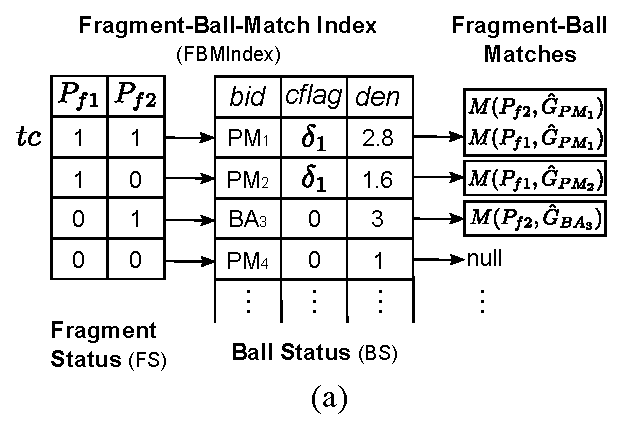
\includegraphics[scale=0.585]{./fig/fig-auxstr-index.eps}}
		\subfigure{\label{fig-inc-maintain-unit}
			\quad\quad \vrule \quad\quad
			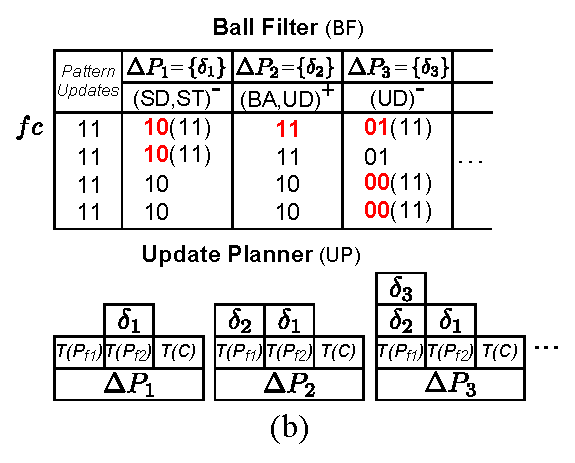
\includegraphics[scale=0.585]{./fig/fig-inc-maintain-unit.eps}}
		\subfigure{\label{fig-inc-maintain-batch}
			\vrule \quad\quad
			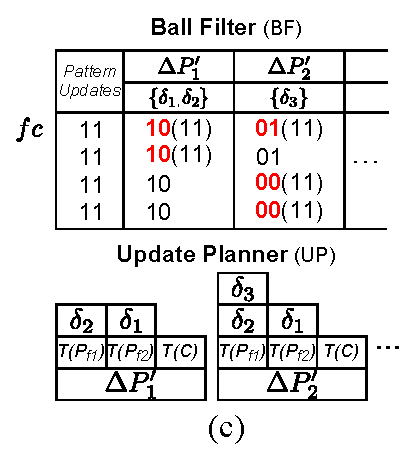
\includegraphics[scale=0.585]{./fig/fig-inc-maintain-batch.eps}}
		\vspace{-3ex}
		\caption{Example auxiliary data structures}
		\label{fig-auxiliary-structures}
		\vspace{-3ex}
	\end{center}
\end{figure*}
%%%%%%%%%%%%%%%%%%%%%%%%%%%%%%%%%%%%%%%%%%%%%
